\section[Системное описание предметной области и постановка задачи]{%
  СИСТЕМНОЕ ОПИСАНИЕ ПРЕДМЕТНОЙ \\
  ОБЛАСТИ И ПОСТАНОВКА ЗАДАЧИ
}\label{sec:spec}

\subsection{Выбор целевой программной платформы}

Для того, чтобы правильно выбрать платформу, для которой
будет разрабатываться мобильное приложение,
следует сначала оценить состояние и перспективы развития
как рынка мобильных устройств связи в целом, так и конкретных
мобильных платформ в частности.
Под состоянием мобильной платформы здесь понимается доля рынка,
занимаемого данной платформой, а под перспективами развития ---
намерения компании-разработчика и сообщества сторонних разработчиков
эту платформу поддерживать.

В целом, современный рынок мобильных устройств можно охарактеризовать
как <<крупный>> и <<быстро развивающийся>>.
По данным ITU, представленным на рисунке~\ref{fig:stat_phone},
за период с 2005 по 2015 год общее число мобильных устройств в мире увеличилось
более чем в три раза и составило более семи миллиардов~\cite{itu_stat_phone}.

\begin{figure}[h!]
  \centering
  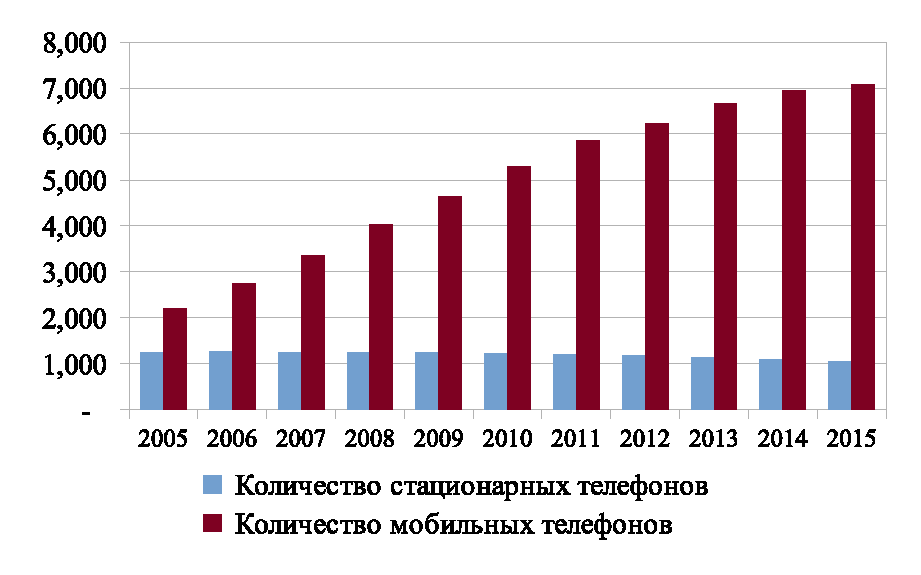
\includegraphics[width=150mm]{fig/stat_phone.eps}
  \caption{Динамика использования персональных устройств связи}
  \label{fig:stat_phone}
\end{figure}

Таким образом, по состоянию на 2015 год, на каждые 100 человек населения земного
шара приходится около 97 мобильных устройств телефонной связи.
Интересно отметить, что общее число станционарных устройств связи
за это время, наоборот, сократилось.

По данным компании Ericsson, в 2015 году было зарегистрировано использование
около 3{,}4 миллиарда смартфонов для доступа в интернет~\cite{ericsson_mobility_report},
что составляет около 47\% от общего числа мобильных устройств.

Популярность различных мобильных платформ сравнивают, как правило,
по объемам продаж устройств, на которых они предустановлены.
По данным агенства Gartner~\cite{gartner_smartphone_stat}, представленным
в таблице~\ref{tbl:gartner_platform_stat}, можно утверждать, что наиболее популярной
мобильной платформой является Android --- мобильная платформа от
компании Google, занимающая на данный момент около 80\% рынка.

\begin{table} [h!]
  \caption{
    Динамика изменения количества проданных смартфонов под
    управлением различных операционных систем
  }\label{tbl:gartner_platform_stat}
    \begin{tabular}{| m{6.6cm} | c | c | c | c |}
      \hline

      \multirow{2}{*}{
      \parbox{6.6cm}{
      \smallskip
      \centering Операционная система
      \smallskip
      }
      }
      & \multicolumn{2}{c|}{
          \parbox{4.5cm}{
            \smallskip
            \centering Четвертый квартал 2014 года
            \smallskip
          }
        }
      & \multicolumn{2}{c|}{
          \parbox{4.5cm}{
            \smallskip
            \centering Четвертый квартал 2015 года
            \smallskip
          }
        } \\
      \cline{2-5}

      & млн. штук & \% & млн. штук & \% \\
      \hline

      Android &  279 & 76 & 325{,}4 & 80{,}7 \\
      \hline

      iOS &  75 & 20{,}4 & 71{,}5 & 17{,}7 \\
      \hline

      Windows & 10{,}5 & 2{,}8 & 4{,}5 & 1{,}1 \\
      \hline

      Blackberry & 1{,}7 & 0{,}4 & 0{,}9 & 0{,}3 \\
      \hline

      Другие & 1{,}3 & 0{,}4 & 0{,}9 & 0{,}2 \\
      \hline

      Всего & 367{,}5 & 100{,}0 & 400{,}6 & 100{,}0 \\
      \hline
    \end{tabular}
\end{table}

Кроме этого, из приведенных данных видно, что Android является единственной
платформой, доля реализованных мобильных устройств под управлением которой
за наблюдаемый период которой не сократилась.

Android позиционируется как бесплатная платформа для широкого круга устройств
любых производителей, что позволяет снизить конечную стоимость устройства,
что, в свою очередь, обуславливает высокую популярность платформы.
Android имеет открытый исходный код; разработчики ядра платформы
охотно принимают патчи от сторонних разработчиков, поэтому вокруг неё сформировалось
активное сообщество.
Приведенные факты позволяют сделать вывод, что платформа Android является наиболее
перспективной для разработки мобильных приложений.

Весьма актуальным является вопрос выбора минимальной версии Android,
которая должна поддерживаться разрабатываемым мобильным приложением.
Дело в том, что различные версии этой платформы не обладают прямой совместимостью.
Действительно, поддержка только новейших версий Android сужает объем потенциальной
целевой аудитории, а поддержка максимального числа версий значительно усложняет
процесс разработки и тестирования.

На рисунке~\ref{fig:stat_android} представлены официальные
данные об относительной популярности различных версий
ОС Android~\cite{google_stat_android}.

\begin{figure}[h!]
  \centering
  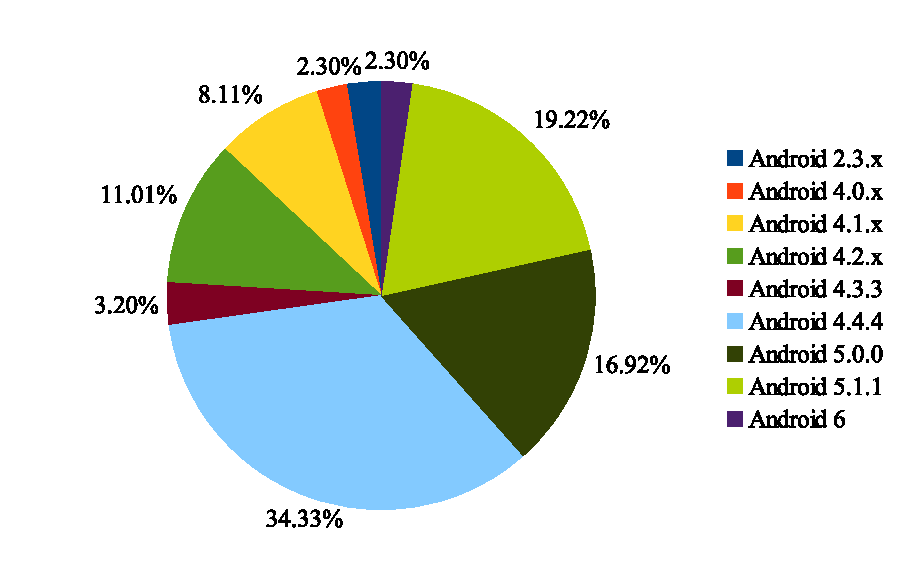
\includegraphics[width=150mm]{fig/stat_android.eps}
  \caption{Относительная популярность различных \\ версий платформы Android}
  \label{fig:stat_android}
\end{figure}

Исходя из этих данных, можно сделать вывод, что наиболее целесообразной
является разработка мобильного приложения для Android версией не ниже 4.0.x.
В этом случае оно будет доступно для 97\% пользователей данной мобильной платформы.


\subsection{Сравнительный анализ существующих приложений-аналогов}

Описание проблем, решаемых данным классом мобильных приложений.
Описание общих требований.
Формирование критериев оценки существующих приложений.

Выделение групп приложений со схожими показателями. Сравнительный анализ типичных представителей этих групп (не менее 3 представителей).

Обзор темы распознавания образов.
Этапы процесса распознавания.
Краткое описание алгоримов, используемых на каждом этапе.

Свободное программное обеспечение. Свободные лицензии. Копилефт.

Постановка задачи проектирования.
Уточнение требований к проектируемому приложению. Ввод данных с использованием камеры.